%% Version 4.3.2, 25 August 2014
%
%%%%%%%%%%%%%%%%%%%%%%%%%%%%%%%%%%%%%%%%%%%%%%%%%%%%%%%%%%%%%%%%%%%%%%
% Template.tex --  LaTeX-based template for submissions to the 
% American Meteorological Society
%
% Template developed by Amy Hendrickson, 2013, TeXnology Inc., 
% amyh@texnology.com, http://www.texnology.com
% following earlier work by Brian Papa, American Meteorological Society
%
% Email questions to latex@ametsoc.org.
%
%%%%%%%%%%%%%%%%%%%%%%%%%%%%%%%%%%%%%%%%%%%%%%%%%%%%%%%%%%%%%%%%%%%%%
% PREAMBLE
%%%%%%%%%%%%%%%%%%%%%%%%%%%%%%%%%%%%%%%%%%%%%%%%%%%%%%%%%%%%%%%%%%%%%

%% Start with one of the following:
% DOUBLE-SPACED VERSION FOR SUBMISSION TO THE AMS
\documentclass{ametsoc}

% TWO-COLUMN JOURNAL PAGE LAYOUT---FOR AUTHOR USE ONLY
% \documentclass[twocol]{ametsoc}

%%%%%%%%%%%%%%%%%%%%%%%%%%%%%%%%
%%% To be entered only if twocol option is used

\journal{waf}

%  Please choose a journal abbreviation to use above from the following list:
% 
%   jamc     (Journal of Applied Meteorology and Climatology)
%   jtech     (Journal of Atmospheric and Oceanic Technology)
%   jhm      (Journal of Hydrometeorology)
%   jpo     (Journal of Physical Oceanography)
%   jas      (Journal of Atmospheric Sciences)	
%   jcli      (Journal of Climate)
%   mwr      (Monthly Weather Review)
%   wcas      (Weather, Climate, and Society)
%   waf       (Weather and Forecasting)
%   bams (Bulletin of the American Meteorological Society)
%   ei    (Earth Interactions)

%%%%%%%%%%%%%%%%%%%%%%%%%%%%%%%%
%Citations should be of the form ``author year''  not ``author, year''
\bibpunct{(}{)}{;}{a}{}{,}

%%%%%%%%%%%%%%%%%%%%%%%%%%%%%%%%

%%% To be entered by author:

%% May use \\ to break lines in title:

\title{Verifying Operational Forecasts of Land-Sea Breeze and Boundary Layer Mixing Processes}

%%% Enter authors' names, as you see in this example:
%%% Use \correspondingauthor{} and \thanks{Current Affiliation:...}
%%% immediately following the appropriate author.
%%%
%%% Note that the \correspondingauthor{} command is NECESSARY.
%%% The \thanks{} commands are OPTIONAL.

    %\authors{Author One\correspondingauthor{Author One, 
    % American Meteorological Society, 
    % 45 Beacon St., Boston, MA 02108.}
% and Author Two\thanks{Current affiliation: American Meteorological Society, 
    % 45 Beacon St., Boston, MA 02108.}}

\authors{Ewan Short\correspondingauthor{School of Earth Sciences, The University of Melbourne, Melbourne, Victoria, Australia.}} 

\email{shorte1@student.unimelb.edu.au}

%% Follow this form:
    % \affiliation{American Meteorological Society, 
    % Boston, Massachusetts.}

\affiliation{School of Earth Sciences, and ARC Centre of Excellence for Climate Extremes, The University of Melbourne, Melbourne, Victoria, Australia.}

%% Follow this form:
    %\email{latex@ametsoc.org}

%\email{}

%% If appropriate, add additional authors, different affiliations:
    %\extraauthor{Extra Author}
    %\extraaffil{Affiliation, City, State/Province, Country}

\DeclareMathOperator{\mse}{mse} 
\DeclareMathOperator{\cov}{cov} 
\DeclareMathOperator{\var}{var} 
\DeclareMathOperator{\pr}{Pr} 

%\extraauthor{}
%\extraaffil{}

%% May repeat for a additional authors/affiliations:

%\extraauthor{}
%\extraaffil{}

%%%%%%%%%%%%%%%%%%%%%%%%%%%%%%%%%%%%%%%%%%%%%%%%%%%%%%%%%%%%%%%%%%%%%
% ABSTRACT
%
% Enter your abstract here
% Abstracts should not exceed 250 words in length!
%
% For BAMS authors only: If your article requires a Capsule Summary, please place the capsule text at the end of your abstract
% and identify it as the capsule. Example: This is the end of the abstract. (Capsule Summary) This is the capsule summary. 

% Run "latexdiff --append-context2cmd="abstract" short18_diurnal_cycles_winds.tex short18_diurnal_cycles_winds_revised.tex > short18_diurnal_cycles_winds_tracked_changes.tex" to track changes

\abstract{Forecasts issued by the Australian Bureau of Meteorology (BoM) are based on automated post-processed model data that is edited by human forecasters. Two types of edits are commonly made to the wind fields. These edits aim to improve how the influences of boundary layer mixing and land-sea breeze processes are represented in the forecast. In this study we compare the diurnally varying component of the BoM's official edited wind forecast, with that of station observations and unedited model datasets, to assess changes to error and bias resulting from these edits. We consider coastal locations across Australia over June, July and August 2018, aggregating data over three spatial scales. The edited forecast generally only produces a lower mean absolute error than model guidance at the coarsest spatial scale (over fifty thousand square kilometres), but can achieve lower seasonal biases over all spatial scales. However, the edited forecast only reduces errors or biases at particular times and locations, and rarely produces lower errors or biases than all model guidance products simultaneously. To better understand the biases in the diurnal wind cycles, we fit modified ellipses to the temporal hodographs of seasonally averaged diurnal wind cycles. Biases in the official forecast diurnal cycle vary with location for multiple reasons, including biases in the directions sea-breezes approach coastlines, amplitude and shape biases in the hodographs, and disagreement as to whether sea-breeze or boundary layer mixing processes contribute most to the diurnal cycle.}

\usepackage{comment}

\begin{document}

\maketitle

\section{Introduction}
\label{Sec:Introduction}
Modern weather forecasts are typically produced by models in conjunction with human forecasters. Forecasters working for the Australian Bureau of Meteorology (BoM) construct a seven day forecast by loading model data into a software package called the Graphical Forecast Editor (GFE), then editing this model data using tools within the GFE. Forecasters working for the United States National Weather Service also use GFE and utilise a similar approach. Forecasters can choose which model to base their forecast on, and refer to this as a choice of \textit{model guidance}. Edits are typically made to account for processes that are under-resolved at the resolutions of the model guidance products, or to correct for perceived biases of the model guidance being used. In Australia, the resulting gridded forecast datasets are provided to the public through the BoM's online MetEye data browser \citep{bomMetEye19}, and are also translated into text and icon forecasts algorithmically. 

Forecasters, and the weather services that employ them, have good reasons for ensuring the diurnally varying component of their wind forecasts are as accurate as possible. In addition to the significant contribution diurnal wind cycles make to overall wind fields \citep[e.g.][]{dai99}, diurnal wind cycles are important for the ventilation of pollution, with sea-breezes transporting clean maritime air inland, where it helps flush polluted air out of the boundary layer \citep{miller03, physick92}. Furthermore, diurnal wind cycles affect the function of wind turbines \citep{englberger18} and the design of wind farms \citep{abkar16}, as daily patterns of boundary layer stability affect turbine wake turbulence, and the losses in wind power that result.

Australian forecasters generally make two types of edits to the surface wind fields on a routine daily basis. The first involves modifying the surface winds after sunrise at locations where the forecaster believes the model guidance is providing a poor representation of boundary layer mixing processes. Boundary layer mixing occurs as the land surface heats up, producing an unstable boundary layer which transports momentum downward to the surface layer. Before this mixing occurs, winds are typically both weaker and ageostrophically oriented due to surface friction \citep{lee18}, and so mixing can affect both the speed and direction of the surface winds. Australian forecasters perform these edits using a GFE tool which allows them to specify a region over which to apply the edit, a height $z$ and a percentage $p$, with the tool then calculating a weighted average of the surface winds and winds at $z$, weighted by $p$.

The second type of edit involves changing the afternoon and evening surface winds around those coastlines where the forecaster believes the model guidance is resolving the sea-breeze poorly. Similarly to with boundary layer mixing, these edits are performed using a GFE tool that allows forecasters to trace out the relevant coastline graphically, choose a wind speed and a time, with the tool then smoothly blending in winds of the given speed perpendicular to the traced coastline at the given time.


To our knowledge, no published work has assessed the diurnal component of human edited forecasts, although some previous studies have assessed the performance of different operational models at specific locations. \citet{svensson11} examined thirty different operational model simulations, including models from most major forecasting centres utilising most commonly used boundary layer parametrisation schemes, and compared their performance with a large eddy simulation (LES), and observations at Kansas, USA, during October 1999. They found that both the models and LES failed to capture the roughly $6$ kn ($1$ kn $\approx 0.514$ m s$^{-1}$) jump in wind speeds shortly after sunrise, and underestimated morning low level turbulence and wind speeds.

Other studies have assessed near-surface wind forecasts, verifying the total wind speeds, not just the diurnal component. \citet{pinson12} studied the 10 m wind speeds from the European Centre for Medium Range Weather Forecasting (ECMWF) operational model ensemble across western Europe over December, January, February 2008/09. They found that the worst performing regions were coastal and mountainous areas, and attributed this to the small scale processes, e.g.~sea and mountain breezes, that are under-resolved by the ensemble's coarse 50 km spatial resolution.

The present study has two goals. First, to describe a method for comparing the diurnal cycles of human edited wind forecasts to those of unedited model guidance forecasts, in order to assess where and when human edits produce a reduction in error or bias. Second, to apply this methodology across Australian coastal locations to assess both boundary layer mixing and land-sea breeze forecaster edits. The remainder of this paper is organised as follows. Section \ref{Sec:Methods} describes the methodology, and datasets to which it is applied, section \ref{Sec:Results} provides results, and sections \ref{Sec:Discussion} and \ref{Sec:Conclusion} provide a discussion and a conclusion, respectively.

\section{Data and Methods} \label{Sec:Methods}
This study compares both human edited and unedited Australian Bureau of Meteorology (BoM) wind forecasts with automatic weather station (AWS) data across Australia. The comparison is performed by first isolating the diurnal perturbations of each dataset by subtracting 24-hour running means, then comparing these perturbations on an hour-by-hour basis.

\begin{figure*}
\centering
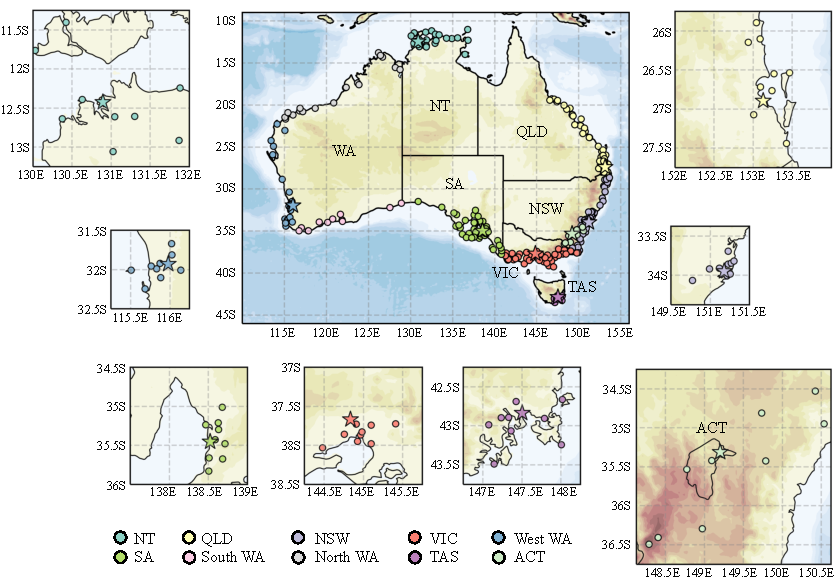
\includegraphics[width=39pc]{old_figures/map.pdf}
\caption{Locations of the automatic weather stations considered in this study, where stars give the locations of the capital city \textit{airport stations}. Stations are divided into the Darwin, Perth, Adelaide, Melbourne, Hobart, Canberra, Sydney and Brisbane \textit{city station groups}, a) to h), respectively, and the \textit{coastal station groups}, i).  Height and depth shading intervals every 200 and 1000 m, respectively.}
\label{Fig:map}
\end{figure*}

\subsection{Data}
Four datasets are considered in this study \citep{shortData19}; the human edited official BoM wind forecast data that is issued to the public, observational data from automatic weather stations (AWS) across Australia, unedited data from the ECMWF's high resolution 10-day forecast model (HRES), and unedited model data from the operational Australian Community Climate and Earth System Simulator (ACCESS), noting that HRES and ACCESS are two of the model guidance products most commonly used by Australian forecasters for winds. We consider just the lead-day one forecasts of the official forecast, HRES and ACCESS, for reasons discussed below. 

This study primarily considers the austral winter months of June, July and August 2018. This short time period was chosen to reduce the effect of changing seasonal and climatic conditions, changing forecasting practice and staff, and of changes to the ACCESS and HRES models. Results for December, January and February 2017/18 are occasionally mentioned to strengthen conclusions or provide a seasonal contrast. 

ACCESS is a nested model: in this study we consider the component covering the Australian region from $65.0^\circ$ south to $16.95^\circ$ north, and $65.0^\circ$ east to $184.57^\circ$ east. This model runs at a $0.11^\circ$ ($\approx 12$ km) horizontal grid spacing, with a standard time-step of $5$ minutes: occasionally a shorter time step of 2.5 minutes is used to overcome numerical instabilities \citep{bom16}. HRES runs at an $\approx 9$ km horizontal grid spacing, with a 7.5 minute time-step \citep{ecmwf19c}. 

Both ACCESS and HRES use parametrisation schemes to simulate sub-grid scale boundary layer turbulence, and the resultant mixing. ACCESS uses the schemes of \citet{lock00} and \citet{louis79} for unstable and stable boundary layers respectively \citep{bom10}. HRES uses similar schemes that the ECMWF develop in-house \citep{ecmwf19a}.

The Bureau's official forecast dataset is produced on a state by state basis at forecasting centres located in most state capitals. To construct the official forecast dataset, forecasters make a choice of model guidance in the GFE, which then interpolates or upscales the model data onto a standard 3 km spatial grid for Victoria and Tasmania, or a 6 km grid for the rest of the country. GFE displays model data at hourly intervals by taking the model guidance output at each hour UTC, with the exception of the HRES model data which is only provided to the BoM at 3 hourly intervals, and is therefore linearly interpolated to hourly intervals by the GFE. Forecasters then make edits to these 3 or 6 km hourly grids to produce the official forecast datasets. 

We therefore compare the official forecast and model guidance datasets as they appear in the GFE, i.e. we compare the upscaled or interpolated datasets on the standardised 3 or 6 km, hourly grids. This both ensures a consistent comparison between model guidance products of different spatial resolutions, and an assessment of how the official forecast compares to the model guidance products as they actually appear to forecasters in the GFE. This is the standard approach the BoM takes when verifying any forecast variable.

These datasets are compared with observations from Australian automatic weather stations (AWS), which typically record wind speed and direction each minute. After basic quality control, 10 minute averages of speed and direction are taken at each station at each hour UTC, usually over the ten minutes leading up to each hour. To calculate verification results, each station is matched with the nearest 3 or 6 km grid-point in the datasets described above.

\subsection{Assessing Diurnal Cycles}
Forecasters edit model guidance wind data to account for under-resolved sea-breeze and boundary layer mixing processes. Instead of attempting to assess each type of edit individually, we study the overall diurnal signal by subtracting a twenty four hour centred running mean \textit{background wind} from each zonal and meridional hourly wind data point, to create wind \emph{perturbation} datasets. 

To compare errors in the official forecast, ACCESS and HRES diurnal cycles we calculate the Euclidean distances between the official or model guidance perturbation vectors at each hour UTC, and the corresponding AWS perturbation vectors at each hour UTC, viewing the Euclidean distance as a measure of absolute error. For example, to assess whether the official forecast perturbations, $\boldsymbol{u}_{\text{O}}$, or ACCESS perturbations, $\boldsymbol{u}_{\text{A}}$, produce lower absolute errors when compared with the observed AWS perturbations, $\boldsymbol{u}_{\text{AWS}}$, we calculate the \textit{difference of absolute errors} (DAE), 
\begin{equation}
\text{DAE}_\text{OA} = \left\lvert \boldsymbol{u}_{\text{AWS}}-\boldsymbol{u}_{\text{A}} \right\rvert - \left\lvert \boldsymbol{u}_{\text{AWS}}-\boldsymbol{u}_{\text{O}} \right\rvert. \label{Eq:DAE}
\end{equation} 
The analogously defined quantities $\text{DAE}_\text{OH}$ and $\text{DAE}_\text{HA}$ provide a comparison of the official forecast and HRES perturbations, and of the HRES and ACCESS perturbations, respectively. We can then take means of the DAE on an hourly basis; i.e.~average all the 00:00 UTC DAE values,  all the 01:00 UTC values, and so forth, and denote such an average by $\overline{\text{DAE}}$. 

Note that $\overline{\text{DAE}}$ compares just \textit{one aspect} of the official forecast with model guidance: it does not, for instance, assess whether the variability of the official forecast is more realistic than that of model guidance. Thus, any statements about performance made throughout this paper refer solely to $\overline{\text{DAE}}$, or subsequently defined metrics, and no claim is being made that these are sufficient to completely characterise the accuracy, or value to the user, of how the diurnal wind cycle is represented in competing forecasts.

Sea-breeze and boundary layer mixing processes depend on the background atmospheric conditions in which they occur. By comparing wind perturbations rather than the overall wind fields we are not claiming these background conditions are irrelevant. However, when a forecaster makes an edit of a wind forecast to better resolve these processes, they are implicitly assuming that future background conditions will be close enough to the preceding 24 hour mean state, or to model predictions of the mean state, to justify making the edit. Thus, it makes sense to compare forecast perturbations to observed perturbations, as long as differences are interpreted as a consequence not only of how the forecaster or model resolves the diurnal cycle, but of how differences in the background state contribute to differences in the perturbations. To minimise the importance of background state differences, this study focuses exclusively on lead-day one forecasts.

Given the large degree of turbulence or random variability in both the AWS, official, and model datasets, care must be taken to ensure we do not pre-emptively conclude the official forecast has outperformed model guidance when $\overline{\text{DAE}}>0$ purely by chance. The method for estimating confidence in $\overline{\text{DAE}}$ is based on a method proposed by \citet{griffiths17}. Time series formed from the DAE values at a particular time, say 00:00 UTC, across the three month time period, are treated as an independent sample of a random variable $E$. The sampling distribution for each $\overline{\text{DAE}}$ can be modelled by a Student's $t$-distribution, and from this we calculate the probability that $E$ is positive, denoted $\pr\left(E > 0\right)$. 

Although temporal autocorrelations of DAE, i.e.~correlations between DAE values at a particular hour from one day to the next, are in practice small or non-existent, they are still accounted for by reducing the ``effective" sample size to $ n \left(1-\rho_1\right)/\left(1+\rho_1\right)$, where $n$ is the actual sample size and $\rho_1$ is the lag-1 autocorrelation \citep{zwiers95,wilks11}. In the language of statistical hypothesis testing, the null hypothesis that $E=0$ would be rejected at significance level $\alpha$ if $\pr(E>0) > 1-\frac{\alpha}{2}$ or $\pr(E<0) > 1-\frac{\alpha}{2}$. However, in this study we prefer to simply state the value of $\pr(E>0)$, referring to this as a \textit{confidence score}, and noting $\pr(E<0) = 1- \pr(E>0)$. We say the official forecast outperforms model guidance with ``high confidence" if $\pr(E>0) \geq 95\%$, or that model guidance outperforms the  official forecast with ``high confidence" if $\pr(E>0) \leq 5\%$, with high confidence implicit whenever it is not explicitly mentioned.

Following the ``fuzzy verification" approach outlined by \citet{ebert08}, forecast and observational perturbation datasets are compared not only at individual stations, but are also averaged over two coarser spatial scales before being compared. The individual stations we consider are the 8 capital city \textit{airport stations}, marked by stars in Fig.~\ref{Fig:map}, as their high operational significance means that they are typically the most well maintained. An intermediate spatial scale is formed by averaging data over the 10 stations closest to each capital city airport station, with some flexibility allowed to ensure stations are roughly parallel to the nearest coastline. These station groups are referred to as the \textit{city station groups}. The coarsest spatial scale is formed by averaging over all stations within 150 km of the nearest coastline, and grouping these by state. The Western Australian coastline is subdivided into three pieces, and stations along the Gulf of Carpentaria, north Queensland Peninsula, and Tasmanian coastlines are neglected, in order to ensure each station group corresponds to an approximately linear segment of coastline to better resolve the land-sea breeze after spatial averaging \citep[e.g.][]{vincent16}. These eight station groups are referred to as the \textit{coastal station groups}. 

To compare errors in the perturbations over the two coarser spatial scales, we modify the definition of DAE in equation (\ref{Eq:DAE}) so that each perturbation dataset is first spatially averaged over either the city or coastal station groups. Confidence scores are calculated for the city and coastal station groups in the same way as for the individual airport stations, treating the spatially averaged data as a single time series. This provides a conservative way to deal with spatial correlation between the stations in each group \citep{griffiths17}. 

To compare biases in the diurnal cycles of each dataset, we calculate the \textit{difference of biases} (DB),
\begin{equation}
\text{DB}_{\text{OA}} = \left\lvert \overline{\boldsymbol{u}}_{\text{AWS}}-\overline{\boldsymbol{u}}_{\text{O}} \right\rvert - \left\lvert \overline{\boldsymbol{u}}_{\text{AWS}}-\overline{\boldsymbol{u}}_{\text{A}} \right\rvert,
\end{equation}
with $\text{DB}_{\text{OH}}$ and $\text{DB}_{\text{HA}}$ defined analogously, where the over-bars denote temporal averages of the perturbations at a particular hour, over June, July and August 2018. These temporally averaged perturbations can be viewed as the climatological diurnal wind cycles over the three month study period for each dataset. Biases over the city and coastal station groups are calculated by taking the spatial average before the temporal average. Uncertainty in the DB is estimated through bootstrapping \citep{efron79}. This is done by performing resampling with replacement on the underlying perturbation datasets, and calculating the DB multiple times using these resampled datasets. This provides a distribution of DB values, which analogously to with DAE, we treat as a sample from a random variable $B$, and use this to estimate $\pr\left(B > 0\right)$.

Another approach to forecast verification is to assess structural features of the phenomena being forecast rather than errors or biases of point predictions; this approach is particularly important at small spatiotemporal scales \citep[e.g.][]{mass02, rife05}. \citet{gille05} obtained summary statistics on the observed structure of mean diurnal wind cycles by using linear regression to calculate the coefficients $u_i$, $v_i$ $i=0,1,2$, for the fits 
\begin{align}
u &= u_0 + u_1 \cos(\omega t) + u_2 \sin(\omega t), \label{Eq:u_h} \\
v &= v_0 + v_1 \sin(\omega t) + v_2 \sin(\omega t), \label{Eq:v_h}
\end{align}
where $\omega$ is the angular frequency of the earth and $t$ is the local solar time in seconds. These fits trace out ellipses in the $x,y$ plane, and descriptive metrics like the eccentricity of the ellipse and the angle the semi-major axis makes with lines of latitude, can be calculated directly from the coefficients $u_1$, $u_2$, $v_1$ and $v_2$. \citet{gille05} applied this fit to scatterometer data, which after temporal averaging resulted in just four zonal and meridional values per location, and as such the fit performed very well.  

However, equations (\ref{Eq:u_h}) and (\ref{Eq:v_h}) do not provide a good fit for the hourly data considered here, primarily because they assume a twelve hour symmetry in the evolution of the diurnal cycle. In practice, asymmetries between daytime heating and nighttime cooling \citep[e.g.][]{svensson11} result in surface wind perturbations accelerating rapidly just after sunrise, but remaining comparatively stagnant at night (e.g.~Fig.~\ref{Fig:clim_hodo}). Thus, we instead fit the equations
\begin{align}
u &= u_0 + u_1 \cos(\alpha(\psi,t)) + u_2 \sin(\alpha(\psi,t)), \label{Eq:u} \\
v &= v_0 + v_1 \sin(\alpha(\psi,t)) + v_2 \sin(\alpha(\psi,t)), \label{Eq:v}
\end{align}
to the climatological perturbations, with $\alpha$ the function from $[0,24) \times [0, 2\pi) \to [0, 2\pi)$ given by
\begin{equation}
\alpha(\psi,t) \equiv \pi \left[\sin\left( \pi \frac{(t - \psi)  \bmod 24}{24} - \frac{\pi}{2} \right) + 1 \right], \label{Eq:alpha}
\end{equation}
with $t$ the time in units of hours UTC, and $\psi$ providing the time when the wind perturbations vary least with time, noting that the same value of $\psi$ is used for both the zonal and meridional perturbations. For each climatological diurnal wind cycle, we solve for the seven parameters $u_0$, $u_1$, $u_2$, $v_0$, $v_1$, $v_2$ and $\psi$ using non-linear regression.

\section{Results}
\label{Sec:Results}
In this section, the methods described in section \ref{Sec:Methods} are applied to Australian forecast and station data over the months of June, July and August 2018. First, differences in absolute errors (DAE) and differences in biases (DB) over this time period are assessed. Second, structural indices are compared to elucidate the physical reasons for biases. 

\begin{figure*}
\centering
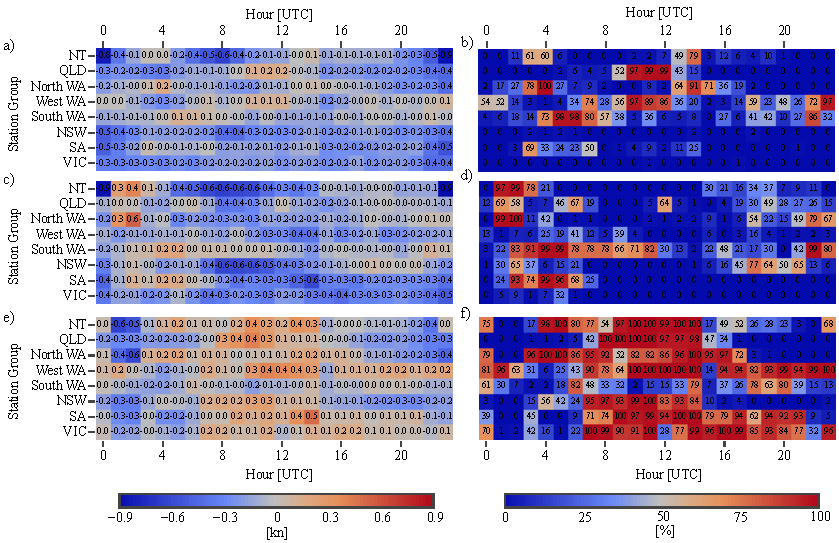
\includegraphics[width=39pc]{old_figures/wpi_coastal.pdf}
\caption{Heatmaps of mean difference of absolute error $\overline{\text{DAE}}$ values, a), c), e), and confidence scores, b), d), f), for each coastal station group (see Fig.~\ref{Fig:map}) and hour of the day, for the official forecast versus ACCESS, a) and b), official forecast versus HRES, c) and d), HRES versus ACCESS, e) and f). Positive $\overline{\text{DAE}}$ values indicate that the former dataset in each pair is on average $\overline{\text{DAE}}$ kn closer to observations than the latter dataset (see equation \ref{Eq:DAE}), where $1$ kn $\approx 0.514$ m s\textsuperscript{-1}. Confidence scores provide the probability the population or ``true" value of $\overline{\text{DAE}}$ is greater than zero (see section \ref{Sec:Methods}).}
\label{Fig:wpi_coastal}
\end{figure*}

\begin{figure}
\centering
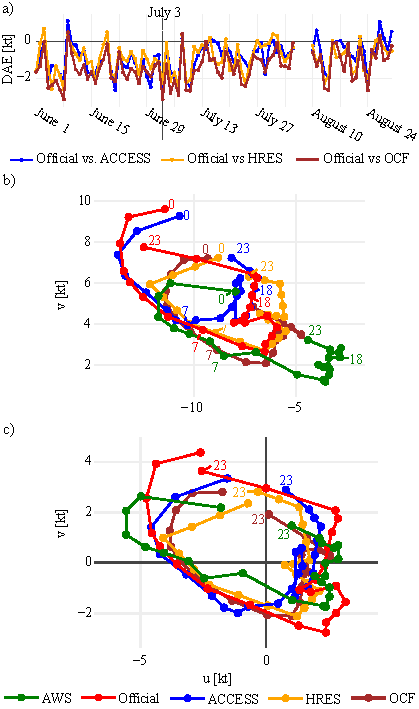
\includegraphics[width=19pc]{old_figures/case_studies_nt.pdf}
\caption{Time series, a), of the difference in absolute error DAE defined in equation (\ref{Eq:DAE}) for the official forecast versus ACCESS, $\text{DAE}_\text{OA}$, and official forecast versus HRES, $\text{DAE}_\text{OH}$, for the NT coastal station group shown in Fig.~\ref{Fig:map} at 23:00 UTC. Also, temporal hodographs in hours UTC showing hourly changes in winds, b), and wind perturbations from a 24 hour running mean, c), at the NT coastal station group on the 3\textsuperscript{rd} of July 2018.}
\label{Fig:case_studies_nt}
\end{figure}

\subsection{Absolute Errors}
\label{Sec:Daily}

Figure \ref{Fig:wpi_coastal} provides the mean difference of absolute error $\overline{\text{DAE}}$ values and confidence scores defined in section \ref{Sec:Methods} for the coastal station groups shown in Fig.~\ref{Fig:map}, for $\overline{\text{DAE}}_\text{OA}$, $\overline{\text{DAE}}_\text{OH}$ and $\overline{\text{DAE}}_\text{HA}$, which represent the official forecast versus ACCESS, official forecast versus HRES, and HRES versus ACCESS comparisons, respectively. The results indicate that for the majority of station groups and hours, both the unedited ACCESS and HRES models outperform the official forecast. The lowest $\overline{\text{DAE}}$ values occur at the NT station group at 23:00 and 00:00 UTC for both $\overline{\text{DAE}}_\text{OA}$ and $\overline{\text{DAE}}_\text{OH}$. Although the official forecast outperforms at least one of ACCESS or HRES at multiple times and station groups, the only group and time where it outperforms both is 05:00 UTC over the South WA station group. HRES generally outperforms ACCESS from 10:00 - 14:00 UTC, with the South WA station group being the main exception.    

Figures \ref{Fig:case_studies_nt} and \ref{Fig:case_studies_wa} provide case studies of the NT and South WA station groups, respectively. Figure \ref{Fig:case_studies_nt} a) provides a time series of DAE for the NT station group at 23:00 UTC. The time series shows significant temporal variability, with DAE frequently dropping below $-2$ kn. Figures \ref{Fig:case_studies_nt} b) and c) show hodographs of the winds and wind perturbations, respectively, at each hour UTC on the 3\textsuperscript{rd} of July, which provides an interesting example. 

Figure \ref{Fig:case_studies_nt} b) shows that the official wind forecast on this day was likely based on edited ACCESS from 00:00 to 06:00 UTC, then edited HRES from 07:00 to 13:00 UTC, then unedited ACCESS from 15:00 to 21:00 UTC. At 22:00 and 23:00 UTC, the official forecast winds acquire stronger east-northeasterly components than the other datasets. Figure \ref{Fig:perth_sounding} a) shows the first ten values from wind soundings at Darwin Airport at 12:00 UTC on July 3\textsuperscript{rd} and 00:00 UTC on July 4\textsuperscript{th}. In both instances the winds are east-southeasterly, and so the rapidly changing wind perturbations at 22:00 UTC in the official forecast likely reflect a boundary layer mixing edit that has been applied either too early, or has strengthened the southeasterly component of the winds too much. Similar issues create low DAE values on the 8\textsuperscript{th} of June and 9\textsuperscript{th} and 10\textsuperscript{th} of July.

Figure \ref{Fig:case_studies_wa} a) provides a time series of DAE for the South WA station group at 05:00 UTC. As with the NT station group there is significant temporal variability, with DAE frequently exceeding 1 kn. Figures \ref{Fig:case_studies_wa} b) and c) provide hodographs of the winds and wind perturbations, respectively, on the 9\textsuperscript{th} of June, another interesting example. The perturbation hodograph shows both HRES and ACCESS under-predicting the amplitude of the diurnal wind cycle on this day. Figure \ref{Fig:perth_sounding} shows wind soundings at Perth Airport, the nearest station to provide wind soundings, between 12:00 UTC on the 8\textsuperscript{th} June and 12:00 UTC on the 9\textsuperscript{th} June. The 8\textsuperscript{th} June 12:00 UTC sounding shows surface northerlies of around $6$ kn, becoming west to northwesterlies of over 20 kn $2.4$ km above the surface. However, the subsequent sounding at 00:00 UTC on the 9\textsuperscript{th} of June shows that the winds acquire a strong northerly component of 30 kn in the first 500 m of the atmosphere, with the final sounding indicating a strong northwesterly wind at 725 m persisting until 12:00 UTC. 

In Fig.~\ref{Fig:case_studies_wa} c), the official forecast perturbations from 04:00 to 07:00 UTC show stronger westerly perturbations than either ACCESS or HRES, improving the amplitude of the official forecast's diurnal wind cycle. However, the AWS perturbations are more northerly than those of the official forecast, and so the official forecast winds have been strengthened in a slightly incorrect direction. One explanation for this discrepancy is that the official forecast has been edited based on the June 8\textsuperscript{th} 12:00 UTC sounding, with the winds above the surface changing direction in the subsequent 12 hours. A similar explanation can be given for the high DAE scores on the  3\textsuperscript{rd} of August, although in this case the official forecast slightly improves both the magnitude and direction of the 05:00 UTC wind perturbations.

\begin{figure}
\centering
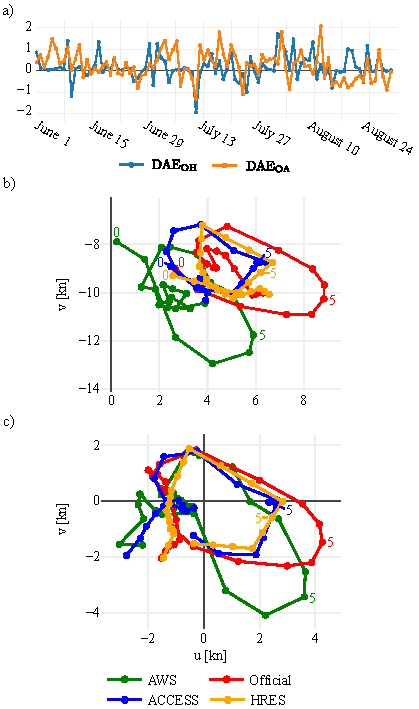
\includegraphics[width=19pc]{old_figures/case_studies_wa.pdf}
\caption{As in Fig.~\ref{Fig:case_studies_nt}, but for, a), the South WA coastal station group at 05:00 UTC, and b) and c), the winds and wind perturbations, respectively, over the South WA coastal station group on the 9\textsuperscript{th} June 2018.} 
\label{Fig:case_studies_wa}
\end{figure}

\begin{figure*}
\centering
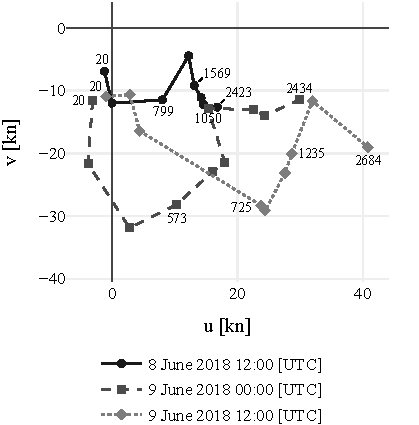
\includegraphics[width=33pc]{old_figures/perth_sounding.pdf}
\caption{Vertical wind soundings at, a), Darwin Airport, and b), Perth Airport, with heights given in metres.}
\label{Fig:perth_sounding}
\end{figure*}

\begin{figure*}
\centering
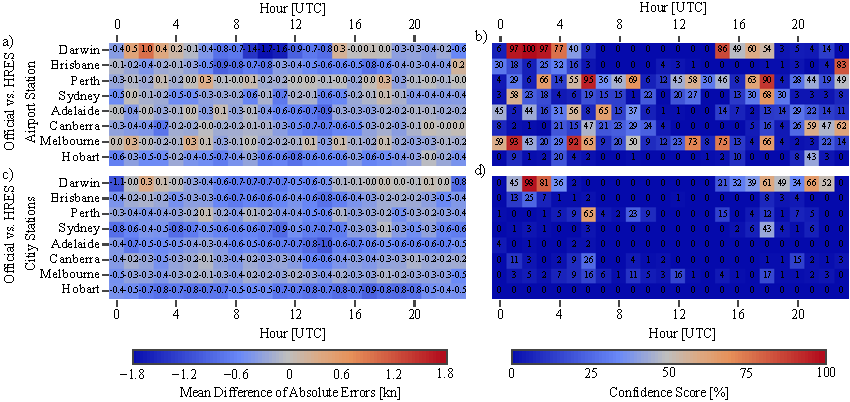
\includegraphics[width=39pc]{old_figures/airport_wpi.pdf}
\caption{As in Fig.~\ref{Fig:wpi_coastal}, but for the official versus HRES mean difference of absolute error $\overline{\text{DAE}}_\text{OH}$ values, a) and c), and confidence scores, b) and d), for the airport stations, a) and b), and city station groups, c) and d).}
\label{Fig:airport_wpi}
\end{figure*}

Fig.~\ref{Fig:airport_wpi} presents the $\overline{\text{DAE}}$ values and confidence scores for the airport stations, and city station groups, for the official forecast versus HRES comparison, i.e.~$\overline{\text{DAE}}_\text{OH}$. The results for the airport stations are noisier than the results for the coastal station groups in Figs.~\ref{Fig:wpi_coastal} c) and d), although they share some similarities. For instance, the official forecast outperforms HRES at 01:00 and 02:00 UTC at both the Darwin airport station and the NT coastal station group. There are four other instances where the official forecast outperforms HRES with at least $90\%$ confidence, although this could simply be occurring by chance due repeated testing \citep[p. 178]{wilks11}.

For the city station groups, HRES outperforms the official forecast almost uniformly. The main exception is the Darwin city station group, where the official forecast outperforms HRES at 02:00 UTC, and there is ambiguity as to whether the official forecast or HRES performs better at 01:00, 03:00 and 04:00 UTC, and from 15:00 to 22:00 UTC. The analogous $\overline{\text{DAE}}_\text{OA}$ official forecast versus ACCESS comparisons (not shown) are similar, with the airport station results noisy, but ACCESS outperforming the official forecast over the city station groups for the vast majority of times and locations. Over the December, January, February 2017/18 season, HRES also outperforms the official forecast almost uniformly over the city station groups, although the official forecast versus ACCESS comparisons are more ambiguous. 

\begin{figure*}
\centering
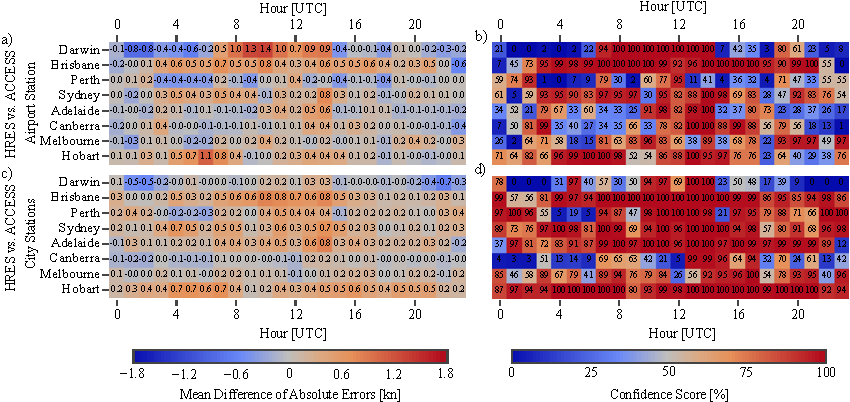
\includegraphics[width=39pc]{old_figures/airport_wpi_EA.pdf}
\caption{As in Fig.~\ref{Fig:airport_wpi}, but for the HRES versus ACCESS mean difference in absolute error $\overline{\text{DAE}}_\text{HA}$ values and confidence scores.
}
\label{Fig:airport_wpi_EA}
\end{figure*}

Figure \ref{Fig:airport_wpi_EA} provides the $\overline{\text{DAE}}$ values and confidence scores for the airport stations, and city station groups, for the HRES versus ACCESS comparison. As with Fig.~\ref{Fig:airport_wpi}, the results for the airport stations are noisy, but more often than not show that HRES outperforms ACCESS. The results for the city station groups show HRES usually outperforms ACCESS, the main exceptions being the Darwin and Canberra city station groups. Results for the December, January, February 2017/18 season are again similar, but here HRES outperforms ACCESS over the city station groups almost uniformly. 

\subsection{Seasonal Biases}
\label{Sec:Seasonal}
Figure \ref{Fig:cwpi_coastal} provides the difference of biases (DB) and confidence scores defined in section \ref{Sec:Methods}, for the coastal station groups for $\text{DB}_\text{OA}$, $\text{DB}_\text{OH}$ and $\text{DB}_\text{HA}$, which represent the the official forecast versus ACCESS, official forecast versus HRES, and HRES versus ACCESS comparisons, respectively. At the NT station at 03:00 UTC, the official forecast outperforms both ACCESS and HRES with confidence $\geq 93\%$. However, both ACCESS and HRES outperform the official forecast at 23:00 and 00:00 UTC, and from 05:00 to 11:00 UTC, consistent with the $\overline{\text{DAE}}$ results of Fig.~\ref{Fig:wpi_coastal}. Figure \ref{Fig:clim_hodo} a) shows that these biases are mostly a consequence of amplitude biases in the official forecast's diurnal cycle.

At the South WA station group from 01:00 to 05:00 UTC, the official forecast outperforms HRES with confidence scores of at least $88\%$. Figure \ref{Fig:clim_hodo} b) shows that HRES underestimates the westerly perturbations at these times, with these perturbations likely associated with boundary layer mixing processes, as discussed in section \ref{Sec:Results} \ref{Sec:Daily}. Each of the official forecast, ACCESS and HRES underestimate the amplitude of the diurnal cycle between 02:00 and 10:00 UTC, including both the westerly perturbations and the southerly sea-breeze perturbations. 

At the NSW station group from 17:00 to 19:00 UTC, the official forecast outperforms both ACCESS and HRES with confidence scores of at least least 95\% and 75\%, respectively. Figure \ref{Fig:clim_hodo} c) shows that these times correspond to ``dimples" in the perturbation temporal hodographs that are present in all four datasets. The official forecast hodograph closely resembles that of ACCESS, except for this dimple, which has been exaggerated relative to ACCESS. Figure \ref{Fig:clim_hodo} c) also shows that although HRES exaggerates the amplitude of the easterly sea-breeze perturbations, it captures the narrower shape of the AWS hodograph better than the official forecast or ACCESS.

At the SA station group from 02:00 to 05:00 UTC and 09:00 to 12:00 UTC, the official forecast outperforms both ACCESS and HRES, although confidence scores do not exceed 88\% and 65\% respectively. Figure \ref{Fig:clim_hodo} d) shows that although the official forecast captures the amplitude of the perturbations from 01:00 to 05:00 UTC almost perfectly, its diurnal cycle is out of phase with that of the AWS during this period, explaining why the official forecast only slightly outperforms ACCESS in the results of Figures \ref{Fig:cwpi_coastal} a) and b).

\begin{figure*}
\centering
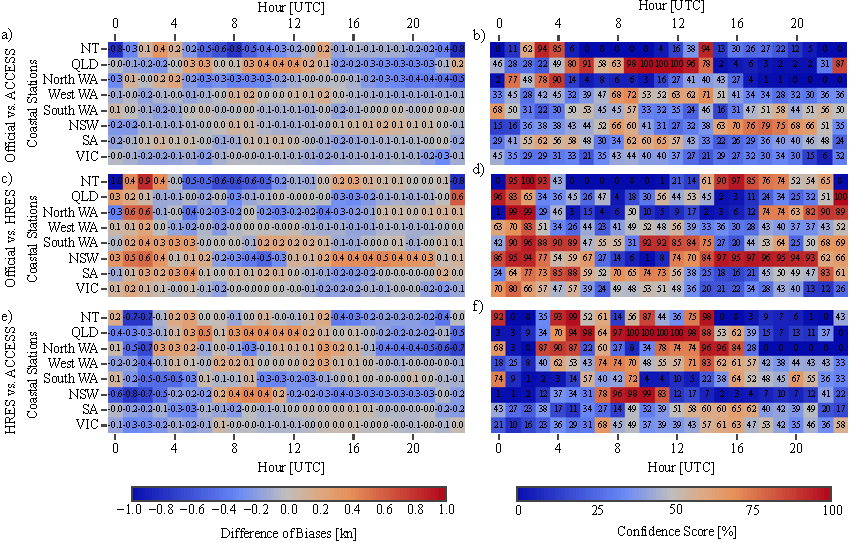
\includegraphics[width=39pc]{old_figures/cwpi_coastal.pdf}
\caption{As in Fig.~\ref{Fig:wpi_coastal}, but for the difference of biases (DB) values and confidence scores.}
\label{Fig:cwpi_coastal}
\end{figure*}

\begin{figure*}
\centering
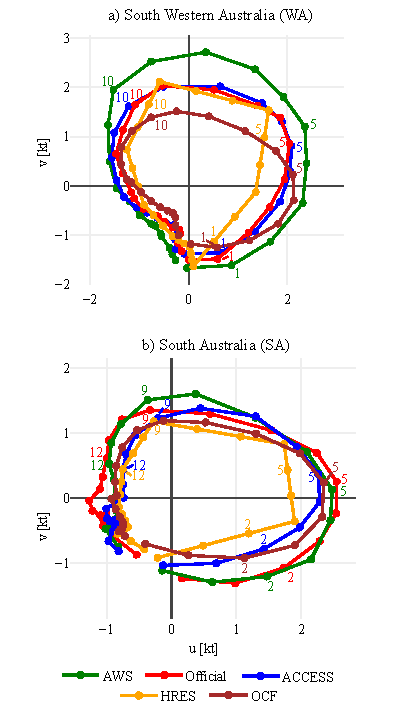
\includegraphics[width=33pc]{old_figures/clim_hodo_alt.pdf}
\caption{Temporal hodographs in hours UTC of wind perturbations spatially averaged over the, a), NT, b) South WA, c) NSW and d), SA coastal station groups (see Fig.~\ref{Fig:map}), and temporally averaged over June, July and August 2018.}
\label{Fig:clim_hodo}
\end{figure*}

\begin{figure*}
\centering
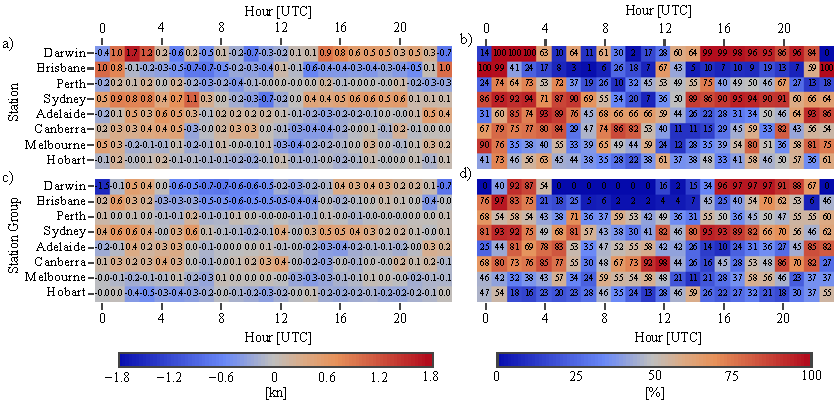
\includegraphics[width=39pc]{old_figures/airport_cwpi.pdf}
\caption{As in Fig.~\ref{Fig:airport_wpi}, but for the difference of biases (DB) values and confidence scores.}
\label{Fig:airport_cwpi}
\end{figure*}

For comparison, Fig.~\ref{Fig:airport_cwpi} presents the DB values and confidence scores for $\text{DB}_\text{OH}$, which represents the official forecast versus HRES comparison, for the airport stations and city station groups. Some regions exhibit consistent results across all three spatial scales, for example, the official forecast is less biased than HRES with at least $80 \%$ confidence at Sydney airport, the Sydney city station group, and the NSW coastal station group, from 14:00 to 18:00 UTC.  

\subsection{Ellipse Fits}

\begin{figure}
\centering
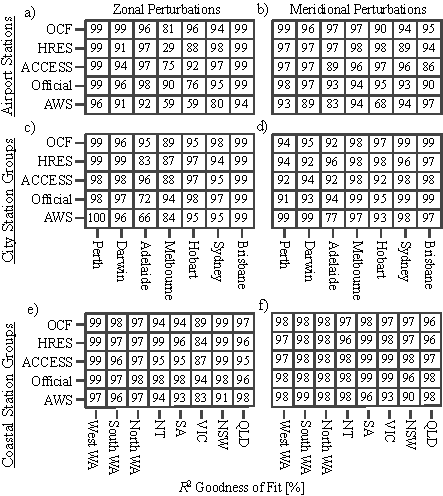
\includegraphics[width=19pc]{old_figures/r_squared.pdf}
\caption{$R^2$ values as percentages for the fit of equation (\ref{Eq:u}) to the zonal perturbations, a), c) and e), and equation (\ref{Eq:v}) to the meridional perturbations, b), d) and f), for the airport stations, a) and b), city station groups, c) and d), and coastal station groups, e) and f), shown in Fig.~\ref{Fig:map}.}
\label{Fig:r_squared}
\end{figure}

The hodographs in Fig.~\ref{Fig:clim_hodo} are roughly elliptical in shape, suggesting that descriptive quantities can be estimated by fitting equations (\ref{Eq:u}) and (\ref{Eq:v}) to the zonal and meridional climatological perturbations, as described in section \ref{Sec:Methods}. Figure \ref{Fig:r_squared} gives the $R^2$ values for the fits of the zonal and meridional perturbations to equations (\ref{Eq:u}) and (\ref{Eq:v}), respectively. The fit performs best at the coastal station group spatial scale, with $R^2$ generally above $95\%$. 

\begin{figure*}
\centering
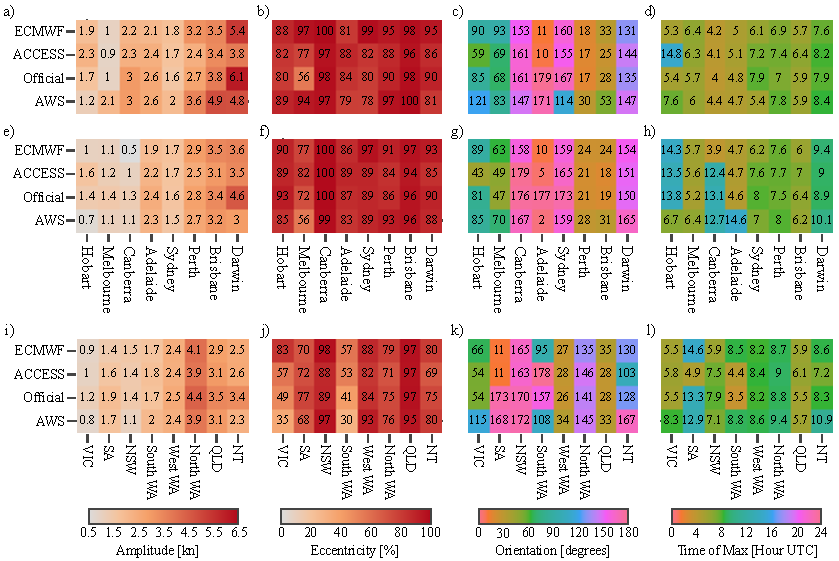
\includegraphics[width=39pc]{old_figures/ellipse_fits.pdf}
\caption{Metrics derived from fitting ellipse equations (\ref{Eq:u}) and (\ref{Eq:v}) to wind perturbations at the Australian capital city airport stations, a) to d), and to wind perturbations spatially averaged over the city station groups and coastal station groups shown in Fig.~\ref{Fig:map}, e) to h) and i) to l) respectively, with perturbations also temporally averaged over June, July and August 2018 in each case. Metrics given are the maximum perturbation speed, a), e) and i), eccentricity of fitted ellipse, b), f) and j), orientation semi-major axis makes with lines of latitude, c), g) and k), and time of maximum perturbation, d), h) and l).}
\label{Fig:ellipse_fits}
\end{figure*}

Figure \ref{Fig:ellipse_fits} provides four descriptive quantities based on the fits of equations (\ref{Eq:u}) and (\ref{Eq:v}) to the averaged perturbations: these are maximum perturbation speed, eccentricity of the fitted ellipse, angle the semi-major axis makes with lines of latitude, and the time at which the maximum perturbation speed is achieved. Fig.~\ref{Fig:ellipse_fits} a) shows that at Brisbane airport the maximum AWS perturbation is at least $1$ kn greater than the official forecast, ACCESS and HRES, and Fig.~\ref{Fig:ellipse_fits} c) shows that the orientation of the AWS fitted ellipse is at least 20 degrees anti-clockwise from the other datasets. Figures \ref{Fig:ellipse_hodo} a) and b) show hodographs of the Brisbane airport climatological perturbations and ellipse fits, respectively. Although the ellipse fits suppress some of the asymmetric details, they capture the amplitudes and orientations of the real climatological diurnal cycles well. In this case the results show that the average AWS sea-breeze approaches from the northeast, whereas the official forecast, HRES and ACCESS sea-breezes approach more from the east-northeast. 

To check whether this just represents a direction bias of the Brisbane Airport weather station, Fig.~\ref{Fig:ellipse_hodo} c) shows the climatological perturbations at the nearby Spitfire Channel station (see Fig.~\ref{Fig:map}). While the amplitude bias is smaller at Spitfire Channel than Brisbane Airport, the directional bias is at least as high. A similar directional bias is evident at the nearby Inner Beacon station (not shown), although the bias is smaller than at Spitfire Channel and Brisbane Airport. Similar biases are also evident at these stations in analogous figures for December, January and February 2017/18 (not shown), with the semi-major axis of the official forecast's ellipse fit oriented $29^\circ$ clockwise from AWS's at Brisbane airport. Figure \ref{Fig:map} shows there are two small islands to the east of Brisbane airport; the more north-northeasterly orientation of the Brisbane Airport sea-breeze suggests these islands may be redirecting winds between the east coast of Brisbane and the west coasts of these islands, and that this local effect is not being captured in the official forecast, ACCESS or HRES. 

\begin{figure*}
\centering
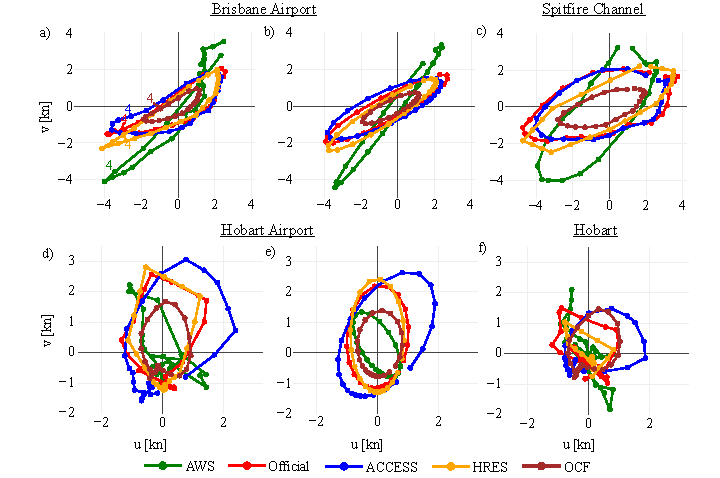
\includegraphics[width=39pc]{old_figures/ellipse_hodo.pdf}
\caption{Temporal hodographs of wind perturbations at each hour UTC averaged over June, July and August 2018, at Brisbane and Hobart airports, a) and d), and the associated ellipse fits, b) and e). For comparison, c) and f) provide the hodographs of the averaged perturbations at the Spitfire Channel and Hobart city stations, respectively (see Fig.~\ref{Fig:map}).}
\label{Fig:ellipse_hodo}
\end{figure*}

Another example is the Hobart Airport station. Figure \ref{Fig:ellipse_fits} c) shows that the semi-major axis of the AWS ellipse fit is oriented 31, 35 and 62 degrees anti-clockwise from the semi-major axes of the HRES, official forecast and ACCESS ellipse fits, respectively. Figures \ref{Fig:r_squared} a) and b) show that the ellipse fit for the AWS perturbations at Hobart airport only achieve $R^2$ values of 59\% and 68\% for the $u$ and $v$ components, respectively, but figures \ref{Fig:ellipse_hodo} d) and e) show that the fit still captures orientations accurately, although it underestimates the maximum AWS perturbation. Figure \ref{Fig:ellipse_hodo} f) provides the climatological perturbations at the Hobart (city) station, which also show a large difference in orientation between ACCESS and AWS. Given the timing of the westerly perturbations in ACCESS, and the fact that the prevailing winds around Tasmania are westerly, these results suggest that ACCESS is exaggerating the boundary layer mixing processes involved in the diurnal cycle around Hobart. These biases are not present during December, January and February 2017/18, as strong south to southeasterly sea-breeze perturbations are now dominant in all four datasets, although the semi-major axis of ACCESS's ellipse fit is still oriented 14 degrees clockwise to that of AWS. 

At the South WA station group (not shown) the semi-major axes of the ACCESS and official forecast ellipse fits are oriented at least 49 degrees anti-clockwise from those of the AWS and HRES ellipse fits, and the HRES perturbations peak between 1.2 and 2.5 hours after the other datasets. These differences occur because eccentricity values are low for this station group, and Figure \ref{Fig:clim_hodo} b) shows that the westerly perturbations associated with boundary layer mixing are weaker for HRES than the other datasets. A similar issue affects the VIC station group, explaining why the semi-major axes of the AWS ellipse fit is oriented at least 49 degrees anti-clockwise from those of the other datasets. 

The Darwin Airport, Darwin Airport station group, and NT station group (not shown) provide further examples. Here the ellipse fits produce favourable $R^2$ values, although the fits slightly underestimate the AWS max perturbation speed at the Darwin Airport station due to this dataset's highly asymmetric hodograph. At all three spatial scales there are timing differences between the perturbation maximums of up to 8.2 hours. These timing differences occur because for some scales and datasets, the later north to northwesterly sea-breeze perturbations dominate the diurnal wind cycle, but for other scales and datasets the earlier easterly to southeasterly boundary layer mixing effects dominate.

\section{Synthesis}
\label{Sec:Discussion}
For land-sea breeze and boundary layer mixing edits to reduce absolute errors in the subsequent days wind forecast, these edits should reduce the absolute errors in the diurnal component of the wind fields. However, Figs.~\ref{Fig:wpi_coastal} and \ref{Fig:airport_wpi} indicate that this is only possible when absolute error is considered at coarse spatial scales, as at individual airport stations results are noisy and ambiguous, and over the intermediate city station group scale HRES outperforms the official forecast almost uniformly.  

Taking the effective resolutions of the models considered in this study to be approximately $7\Delta x$ \citep[e.g.][]{skamarock04, abdalla13}, where $\Delta x$ is the horizontal grid spacing, we have effective resolutions of $\approx 84$ km and $\approx 63$ km for ACCESS and HRES respectively. From resolution considerations alone, one might expect that forecaster edits would be able to reduce errors at the individual airport station scale, and the intermediate city station group scale (see Fig.~\ref{Fig:map}), as motion at these scales is unresolved or only partially resolved by ACCESS and HRES. 

To further investigate the effect of spatial scale on error, consider first just the zonal components of the AWS and official forecast wind perturbations, denoted by $u_\text{AWS}$ and $u_\text{O}$ respectively. Considering just the values at a particular hour UTC, over the entire June, July, August time period, the mean square error $\mse\left(u_\text{AWS}, u_\text{O}\right) = \overline{\left(u_\text{AWS} - u_\text{O}\right)^2}$ can be decomposed $\mse\left(u_\text{AWS}, u_\text{O}\right)=$ 
\begin{equation}
\underbrace{\var\left(u_\text{AWS}\right) + \var\left(u_\text{O}\right) - 2\cov\left(u_\text{AWS}, u_\text{O}\right)}_\text{error variance} + \underbrace{\left(\overline{u}_\text{AWS} - \overline{u}_\text{O}\right)^2}_{\text{squared bias}} \label{Eq:MSE}
\end{equation}
where $\var$, $\cov$ and the over-bar denote the sample variance, covariance and mean respectively. The first three terms are the variance of $u_\text{AWS} - u_\text{O}$, i.e. the error variance, and the last term is the square of the bias between $u_\text{AWS}$ and $u_\text{O}$. Equation (\ref{Eq:MSE}) can also be applied to the MSEs of HRES. Note that the mean square errors (MSEs) of the official forecast and HRES are closely related to $\overline{\text{DAE}}_\text{OH}$, which is the difference between the mean absolute errors of the official forecast and HRES; similarly, the squared bias components of the MSEs are closely related to $\text{DB}_\text{OH}$. 

\begin{figure*}
\centering
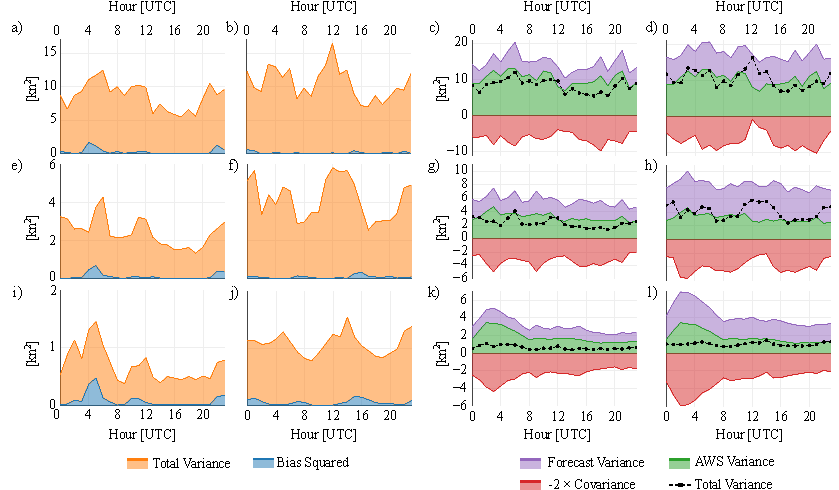
\includegraphics[width=39pc]{old_figures/error_decomp_sa.pdf}
\caption{Mean square error between the AWS and HRES zonal perturbations $\overline{\left(u_\text{AWS} - u_\text{H}\right)^2}$, a), e), and i), decomposed into the error variance $\var\left(u_\text{AWS} - u_\text{H}\right)$ and squared bias $\left(\overline{u}_\text{AWS} - \overline{u}_\text{H}\right)^2$ terms of equation (\ref{Eq:MSE}). Also, the decomposed mean square error between the AWS and official forecast zonal perturbations, b), f) and j). Additionally, the HRES and AWS error variance term $\var\left(u_\text{AWS} - u_\text{H}\right)$ decomposed into the $\var\left(u_\text{AWS}\right)$, $\var\left(u_\text{H}\right)$ and  $- 2 \cdot \cov\left(u_\text{AWS}, u_\text{H}\right)$ terms, c), g) and k), and analogously for the official forecast and AWS error variance term $\var\left(u_\text{AWS} - u_\text{O}\right)$, d), h) and l). Decompositions given for Adelaide Airport, a) to d), the Adelaide city station group, e) to h), and the SA coastal station group, i) to l) (see Fig.~\ref{Fig:map}.)}
\label{Fig:error_decomp_sa}
\end{figure*}

Figure \ref{Fig:error_decomp_sa} shows the terms of equation (\ref{Eq:MSE}) for both the official forecast and HRES for Adelaide Airport, the Adelaide city station group, and the SA coastal station group.  At all three scales the official forecast varies more than HRES, which is also the case at the other locations considered in this study. At Adelaide airport the variance of AWS is significantly larger than either the official forecast or HRES, but this additional variability is mostly uncorrelated to either dataset. This is unsurprising from representation considerations alone \citep[e.g.][]{zaron06}, as the official forecast and HRES data represent averages over 6 km spatial grid-cells, whereas the AWS data represent point values. As a result, error variance terms are much larger than the squared bias terms, and of comparable magnitudes for both datasets. This is consistent with the comparatively noisy DAE results of Figs.~\ref{Fig:airport_wpi} a) and b). 

At the intermediate Adelaide city station group scale, the AWS variances are of similar magnitudes to those of HRES, but smaller than those of the official forecast, with the official forecast's additional variability mostly uncorrelated to AWS. This results in larger error variance terms for the official forecast, consistent with HRESs almost complete outperformance of the official forecast in Figs.~\ref{Fig:airport_wpi} c) and d). Over the coarse SA coastal station group scale, variances in all three datasets are now small enough that the error variance terms no longer dwarf the bias terms. Although the error variance of the official forecast is still larger than that of HRES, HRES's zonal biases at 05:00 UTC are now sufficient to result in a larger MSE at this time, consistent with the DAE results of Fig.~\ref{Fig:wpi_coastal} c) and d). 

Analogous points can be made for the other locations considered in this study, the main exception being Darwin airport, Darwin city station group, and the NT coastal station group, where zonal biases in HREF around 01:00 - 03:00 UTC are large enough to overcome the official forecast's larger error variance, producing the results of Fig.~\ref{Fig:airport_wpi} and Figs.~\ref{Fig:wpi_coastal} c) and d). The results of Fig.~\ref{Fig:airport_wpi} c) and d) are therefore generally a consequence of the official forecast being more variable than HRES, with this additional variability mostly random, in the sense of being uncorrelated with AWS. Similarly, the official forecast is generally more variable than ACCESS, explaining why the official forecast also struggles to outperform ACCESS at these scales, and ACCESS is generally more variable than HRES, explaining why HRES generally outperforms ACCESS in the DAE results of Fig.~\ref{Fig:airport_wpi_EA}. In the coastal station group DAE results of Fig.~\ref{Fig:wpi_coastal}, the random variability in each dataset is reduced, and biases are now large enough to actually affect errors in the diurnal component of the forecast.  

These results show that switching model guidance products or performing edits can add more random noise to the diurnal component of the official forecast than what can be offset by reductions in bias, or improved correlations with AWS. Because the official forecast is built from multiple model datasets, most commonly HRES and ACCESS, blending datasets with different means will tend to produce greater variance than any of the component datasets. If the choice of model guidance is made primarily on which model best captures more slowly evolving synoptic scale features, then switching model guidance may add random variability to the diurnal component of the official forecast. Furthermore, unless all forecasters follow identical thought processes when making edits, the edits will also add random variability. It is less clear why ACCESS shows greater random variability than HRES: one cause may be ACCESS's shorter time-step.  

These results have implications for forecasting practice. Model guidance products are indeed biased in how they resolve diurnal wind cycles (e.g. Fig.~\ref{Fig:ellipse_hodo}), and there is therefore scope for forecaster edits to reduce these biases. However, editing model guidance generally fails to reduce error in the forecast diurnal cycle, even at scales finer than the effective resolutions of the models, as the cycle itself is mostly hidden by random variability. Averaging over large areas reduces this random variability, and so biases have a greater impact on forecast error, but even at large scales Fig.~\ref{Fig:wpi_coastal} shows model guidance still outperforms the official forecast more often than not. 

Reducing the random variability of the official forecast, or the model guidance datasets that comprise it, will therefore improve the capacity of these types of edits to reduce error. One way to do this would be to move to an ensemble forecasting system, another would be to post process model guidance products, such as by averaging multiple time steps around the hour, before including them in GFE. 

\section{Conclusion}
\label{Sec:Conclusion}
In this study we have presented methods for verifying the diurnal component of wind forecasts, with the intended application being the assessment of the edits Australian forecasters make to model guidance datasets in order to better resolve land-sea breeze and boundary layer mixing processes. We considered both errors and seasonal biases at each hour UTC, over three spatial scales, but the methods are immediately generalisable to other spatiotemporal scales. 

When the methods are applied to Australian forecast data, the results indicate that the official edited forecast only produces lower absolute errors in the diurnal wind cycle when averaged over coarse spatial scales of $500\times 150$ km$^{2}$ to $2000 \times 150$ km$^{2}$: this scale corresponds to the aggregation of data within 150 km of the Australian coastline, subdivided into linear segments of coastline and by state (see Fig.~\ref{Fig:map}). Even at these scales, reductions in error are isolated to particular locations and times of day, and the official forecast rarely has lower mean absolute error than both commonly used model guidance products simultaneously. This suggests that forecaster skill in improving diurnal wind processes lies more in making the choice of model guidance than in making edits.

By contrast, the official forecast can produce lower seasonal biases than model guidance at all three spatial scales, but again, it rarely produces lower biases than both standard model guidance products simultaneously. Reduced seasonal biases do not translate into reduced errors at the two smaller spatial scales because the diurnal cycle is mostly masked by the random variability in each dataset. Furthermore, because the official forecast exhibits much greater random variability than HRES, HRES almost uniformly outperforms the official forecast over the intermediate $50\times 50$ km$^{2}$ to $200 \times 200$ km$^{2}$ spatial scale. The same is true for ACCESS, although to a slightly lesser extent, and also explains why HRES mostly outperforms ACCESS at this scale. 

We also compare structural features of the diurnal wind cycles of each dataset by fitting modified ellipses to hodographs of seasonally averaged diurnal wind cycles, then deriving metrics from these ellipses. This approach reveals structural biases in the official forecast, including directional biases in the approach of the sea-breeze at Brisbane airport, eccentricity biases along the coast of NSW, and amplitude biases along the southwest coast of WA. It also reveals biases in model guidance datasets, such as ACCESS's overemphasis of boundary layer mixing processes around Hobart.   

Future research could extend this study in multiple directions. One important question is whether the random variability in the official forecast, or the model guidance products that comprise it, could be reduced through ensemble forecasting or post-processing, as reducing random variability would both decrease errors, and increase the value of land-sea breeze and boundary layer mixing edits. Another goal could be to identify precisely the spatiotemporal scales at which diurnal wind cycles can be identified against background noise, so as to better understand the scales at which land-sea breeze and boundary layer mixing edits can add value to a forecast.  

\acknowledgments
Funding for this study was provided for Ewan Short by the Australian Research Council's Centre of Excellence for Climate Extremes (CE170100023). Datasets and software were generously provided by the Australian Bureau of Meteorology's Evidence Targeted Automation team, with additional code available online \citep{shortGitVeri19}. Thanks are due to Michael Foley, Deryn Griffiths, Nicholas Loveday, Ben Price and Alexei Hider for providing support at the Bureau of Meteorology's Melbourne and Darwin offices, and to Professors Craig Bishop and Todd Lane from the University of Melbourne, and Carly Kovacik from the United States' National Weather Service, for some helpful conversations. 
\bibliographystyle{ametsoc2014}
\bibliography{./references.bib}

\end{document}
